%% BioMed_Central_Tex_Template_v1.06
%%                                      %
%  bmc_article.tex            ver: 1.06 %
%                                       %

%%IMPORTANT: do not delete the first line of this template
%%It must be present to enable the BMC Submission system to
%%recognise this template!!

%%%%%%%%%%%%%%%%%%%%%%%%%%%%%%%%%%%%%%%%%
%%                                     %%
%%  LaTeX template for BioMed Central  %%
%%     journal article submissions     %%
%%                                     %%
%%          <8 June 2012>              %%
%%                                     %%
%%                                     %%
%%%%%%%%%%%%%%%%%%%%%%%%%%%%%%%%%%%%%%%%%


%%%%%%%%%%%%%%%%%%%%%%%%%%%%%%%%%%%%%%%%%%%%%%%%%%%%%%%%%%%%%%%%%%%%%
%%                                                                 %%
%% For instructions on how to fill out this Tex template           %%
%% document please refer to Readme.html and the instructions for   %%
%% authors page on the biomed central website                      %%
%% http://www.biomedcentral.com/info/authors/                      %%
%%                                                                 %%
%% Please do not use \input{...} to include other tex files.       %%
%% Submit your LaTeX manuscript as one .tex document.              %%
%%                                                                 %%
%% All additional figures and files should be attached             %%
%% separately and not embedded in the \TeX\ document itself.       %%
%%                                                                 %%
%% BioMed Central currently use the MikTex distribution of         %%
%% TeX for Windows) of TeX and LaTeX.  This is available from      %%
%% http://www.miktex.org                                           %%
%%                                                                 %%
%%%%%%%%%%%%%%%%%%%%%%%%%%%%%%%%%%%%%%%%%%%%%%%%%%%%%%%%%%%%%%%%%%%%%

%%% additional documentclass options:
%  [doublespacing]
%  [linenumbers]   - put the line numbers on margins

%%% loading packages, author definitions

\documentclass[twocolumn]{bmcart}% uncomment this for twocolumn layout and comment line below
%\documentclass{bmcart}

%%% Load packages
%\usepackage{amsthm,amsmath}
%\RequirePackage{natbib}
%\RequirePackage[authoryear]{natbib}% uncomment this for author-year bibliography
%\RequirePackage{hyperref}
\usepackage[utf8]{inputenc} %unicode support
%\usepackage[applemac]{inputenc} %applemac support if unicode package fails
%\usepackage[latin1]{inputenc} %\UNIX support if unicode package fails
\usepackage{ragged2e}
\usepackage[english]{babel}
\usepackage{graphicx}



%%%%%%%%%%%%%%%%%%%%%%%%%%%%%%%%%%%%%%%%%%%%%%%%%
%%                                             %%
%%  If you wish to display your graphics for   %%
%%  your own use using includegraphic or       %%
%%  includegraphics, then comment out the      %%
%%  following two lines of code.               %%
%%  NB: These line *must* be included when     %%
%%  submitting to BMC.                         %%
%%  All figure files must be submitted as      %%
%%  separate graphics through the BMC          %%
%%  submission process, not included in the    %%
%%  submitted article.                         %%
%%                                             %%
%%%%%%%%%%%%%%%%%%%%%%%%%%%%%%%%%%%%%%%%%%%%%%%%%


%\def\includegraphic{}
%\def\includegraphics{}



%%% Put your definitions there:
\startlocaldefs
\endlocaldefs


%%% Begin ...
\begin{document}

%%% Start of article front matter
\begin{frontmatter}

\begin{fmbox}
\dochead{Research}

%%%%%%%%%%%%%%%%%%%%%%%%%%%%%%%%%%%%%%%%%%%%%%
%%                                          %%
%% Enter the title of your article here     %%
%%                                          %%
%%%%%%%%%%%%%%%%%%%%%%%%%%%%%%%%%%%%%%%%%%%%%%

\title{Association of variants in gene coding regions with clinical data in colombian patients using data mining}

%%%%%%%%%%%%%%%%%%%%%%%%%%%%%%%%%%%%%%%%%%%%%%
%%                                          %%
%% Enter the authors here                   %%
%%                                          %%
%% Specify information, if available,       %%
%% in the form:                             %%
%%   <key>={<id1>,<id2>}                    %%
%%   <key>=                                 %%
%% Comment or delete the keys which are     %%
%% not used. Repeat \author command as much %%
%% as required.                             %%
%%                                          %%
%%%%%%%%%%%%%%%%%%%%%%%%%%%%%%%%%%%%%%%%%%%%%%

\author[
   addressref={aff1},                   % id's of addresses, e.g. {aff1,aff2}
   corref={aff1},                       % id of corresponding address, if any
   noteref={n1},                        % id's of article notes, if any
   email={jevelezse@unal.edu.co}   % email address
]{\inits{JV}\fnm{Jennifer} \snm{Velez}}
\author[
   addressref={aff2},
   email={eleonguz@unal.edu.co}
]{\inits{EL}\fnm{Elizabeth} \snm{Leon}}

%%%%%%%%%%%%%%%%%%%%%%%%%%%%%%%%%%%%%%%%%%%%%%
%%                                          %%
%% Enter the authors' addresses here        %%
%%                                          %%
%% Repeat \address commands as much as      %%
%% required.                                %%
%%                                          %%
%%%%%%%%%%%%%%%%%%%%%%%%%%%%%%%%%%%%%%%%%%%%%%

\address[id=aff1]{%                           % unique id
  \orgname{School of Engineering, Universidad Nacional de Colombia}, % university, etc
  %\street{},                     %
  %\postcode{}                                % post or zip code
  \city{Bogotá D.C.},                              % city
  \cny{Colombia}                                    % country
}
\address[id=aff2]{%
  \orgname{School of Engineering, Universidad Nacional de Colombia},
  %\street{D\"{u}sternbrooker Weg 20},
  %\postcode{24105}
  \city{Bogotá D.C},
  \cny{Colombia}
}

%%%%%%%%%%%%%%%%%%%%%%%%%%%%%%%%%%%%%%%%%%%%%%
%%                                          %%
%% Enter short notes here                   %%
%%                                          %%
%% Short notes will be after addresses      %%
%% on first page.                           %%
%%                                          %%
%%%%%%%%%%%%%%%%%%%%%%%%%%%%%%%%%%%%%%%%%%%%%%

\begin{artnotes}
%\note{Sample of title note}     % note to the article
\note[id=n1]{Equal contributor} % note, connected to author
\end{artnotes}

%\end{fmbox}% comment this for two column layout

%%%%%%%%%%%%%%%%%%%%%%%%%%%%%%%%%%%%%%%%%%%%%%
%%                                          %%
%% The Abstract begins here                 %%
%%                                          %%
%% Please refer to the Instructions for     %%
%% authors on http://www.biomedcentral.com  %%
%% and include the section headings         %%
%% accordingly for your article type.       %%
%%                                          %%
%%%%%%%%%%%%%%%%%%%%%%%%%%%%%%%%%%%%%%%%%%%%%%

\begin{abstractbox}

\begin{abstract} % abstract
\parttitle{Background} %if any
\justify
The need to understand the biological processes that are involved in different diseases, from the available biological data such as genomic sequences, microarrays, protein interactions, biomedical images among others and the rapid adoption of electronic medical records that provides an opportunity for large-scale research . Therefore, data mining techniques for the discovery of knowledge from obtaining information from different sources are increasingly important in biological and medical research.

\parttitle{Results} %if any
A group model was implemented for 228 patients, and they were associated with the variants for 4813 genes, obtaining 5 groups with their options available in the rules. As an analysis, an analysis of the CFTR
the gene was also carried out by means of association rules and previously obtained groups. This is the search tag the measurements of the frequencies of the population were made in terms of the number of variants present the age, sex, type of variant and the allelic state of the variants. It was found that for the CFTR hay gene without pathogenic variants in the sampled population. A board also created to visualize the groups and the necessary rules for group and a database for variants in exons for Colombian patients.

\parttitle{Conclusions} %if any
Data mining techniques applied to disk support allow an inference of genetics structure the Colombian population and the epidemiological follow-up of the variants and their possible effects in patient's phenotypes.
\end{abstract}

%%%%%%%%%%%%%%%%%%%%%%%%%%%%%%%%%%%%%%%%%%%%%%
%%                                          %%
%% The keywords begin here                  %%
%%                                          %%
%% Put each keyword in separate \kwd{}.     %%
%%                                          %%
%%%%%%%%%%%%%%%%%%%%%%%%%%%%%%%%%%%%%%%%%%%%%%

\begin{keyword}
\kwd{Variant}
\kwd{data mining}
\kwd{clustering}
\kwd{association rules}
\end{keyword}

% MSC classifications codes, if any
%\begin{keyword}[class=AMS]
%\kwd[Primary ]{}
%\kwd{}
%\kwd[; secondary ]{}
%\end{keyword}

\end{abstractbox}
%
\end{fmbox}% uncomment this for twcolumn layout

\end{frontmatter}

%%%%%%%%%%%%%%%%%%%%%%%%%%%%%%%%%%%%%%%%%%%%%%
%%                                          %%
%% The Main Body begins here                %%
%%                                          %%
%% Please refer to the instructions for     %%
%% authors on:                              %%
%% http://www.biomedcentral.com/info/authors%%
%% and include the section headings         %%
%% accordingly for your article type.       %%
%%                                          %%
%% See the Results and Discussion section   %%
%% for details on how to create sub-sections%%
%%                                          %%
%% use \cite{...} to cite references        %%
%%  \cite{koon} and                         %%
%%  \cite{oreg,khar,zvai,xjon,schn,pond}    %%
%%  \nocite{smith,marg,hunn,advi,koha,mouse}%%
%%                                          %%
%%%%%%%%%%%%%%%%%%%%%%%%%%%%%%%%%%%%%%%%%%%%%%

%%%%%%%%%%%%%%%%%%%%%%%%% start of article main body
% <put your article body there>

%%%%%%%%%%%%%%%%
%% Background %%
%%
\section*{Content}
This paper is organized in section Background, Results ,Discussion, Conclusions and Methods. %\cite{koon,oreg,khar,zvai,xjon,schn,pond,smith,marg,hunn,advi,koha,mouse}

\section*{Background}
Biological data mining (seen from bioinformatics) is the process of extracting new knowledge (previously unknown) from biological data, this also allows the use of concepts of data mining and automatic learning in theories and applications in research Biological, by deeding the data that are used to be applied, are genomes that come from DNA sequencing, transcriptome sequences that are RNA or proteins that come from inferences and experimental data from chemistry \cite{Farid2016}.

Inferences regarding large amounts of genomic data require analysis of computational tools to interpret data, being one of the most active areas where data mining is used (I understand data mining as the method of extracting information through learning automatic, statistics, artificial intelligence, recognition and visualization patterns) to solve biological problems, some examples where mining techniques have been applied is the classification of genes, the analysis of mutations in cancer and gene expression \cite{Littlefield}.

Clustering techniques of differentially expressed genes have also been applied, vector support machines have been used to associate the interactions between genes and generate biological networks, as well as traditional methodologies for data mining are not precise or efficient and they require new algorithms to be developed and methodologies that respond in a more precise way to a biological question \cite{Zaki2007}. Without forgetting that it is necessary to evaluate the available platforms, the technological tools that allow the implementation of processes that associate data with research and obtain
more generalized results. This should apply to the research requirements to ensure successful implementation \cite{Zaki2007}.

Some of the data mining tasks are: 1. Classification: where the data is classified to a predefined class, 2. Association: see elements that are associated by rules, 3. Grouping or grouping: as the definition of a population of data within a subgroup or group \cite{Littlefield}.

The use of high performance sequencing techniques together with the application of data mining can contribute to the diagnosis of complex diseases such as cancer\cite{Hannah-Shmouni2015,Kawashima2017}.
\section*{Results}
\subsection*{Exploratory analysis}
The exploratory analysis of the information contained in the database was carried out. A sample of 250 patients donated by the Genetix SA laboratory was taken, of which only 228 had the informed consent to use the information for research purposes.

\begin{figure}[h!]
	\centering
	\includegraphics[width=0.3\textwidth]{/home/jennifer/Documentos/latex1/Plantilla_LaTex_UN/Kap4/general}
	\caption{Distribution of age range and gender of patients}
	\label{fig:general}
\end{figure}

\begin{figure}[h!]
	\centering
	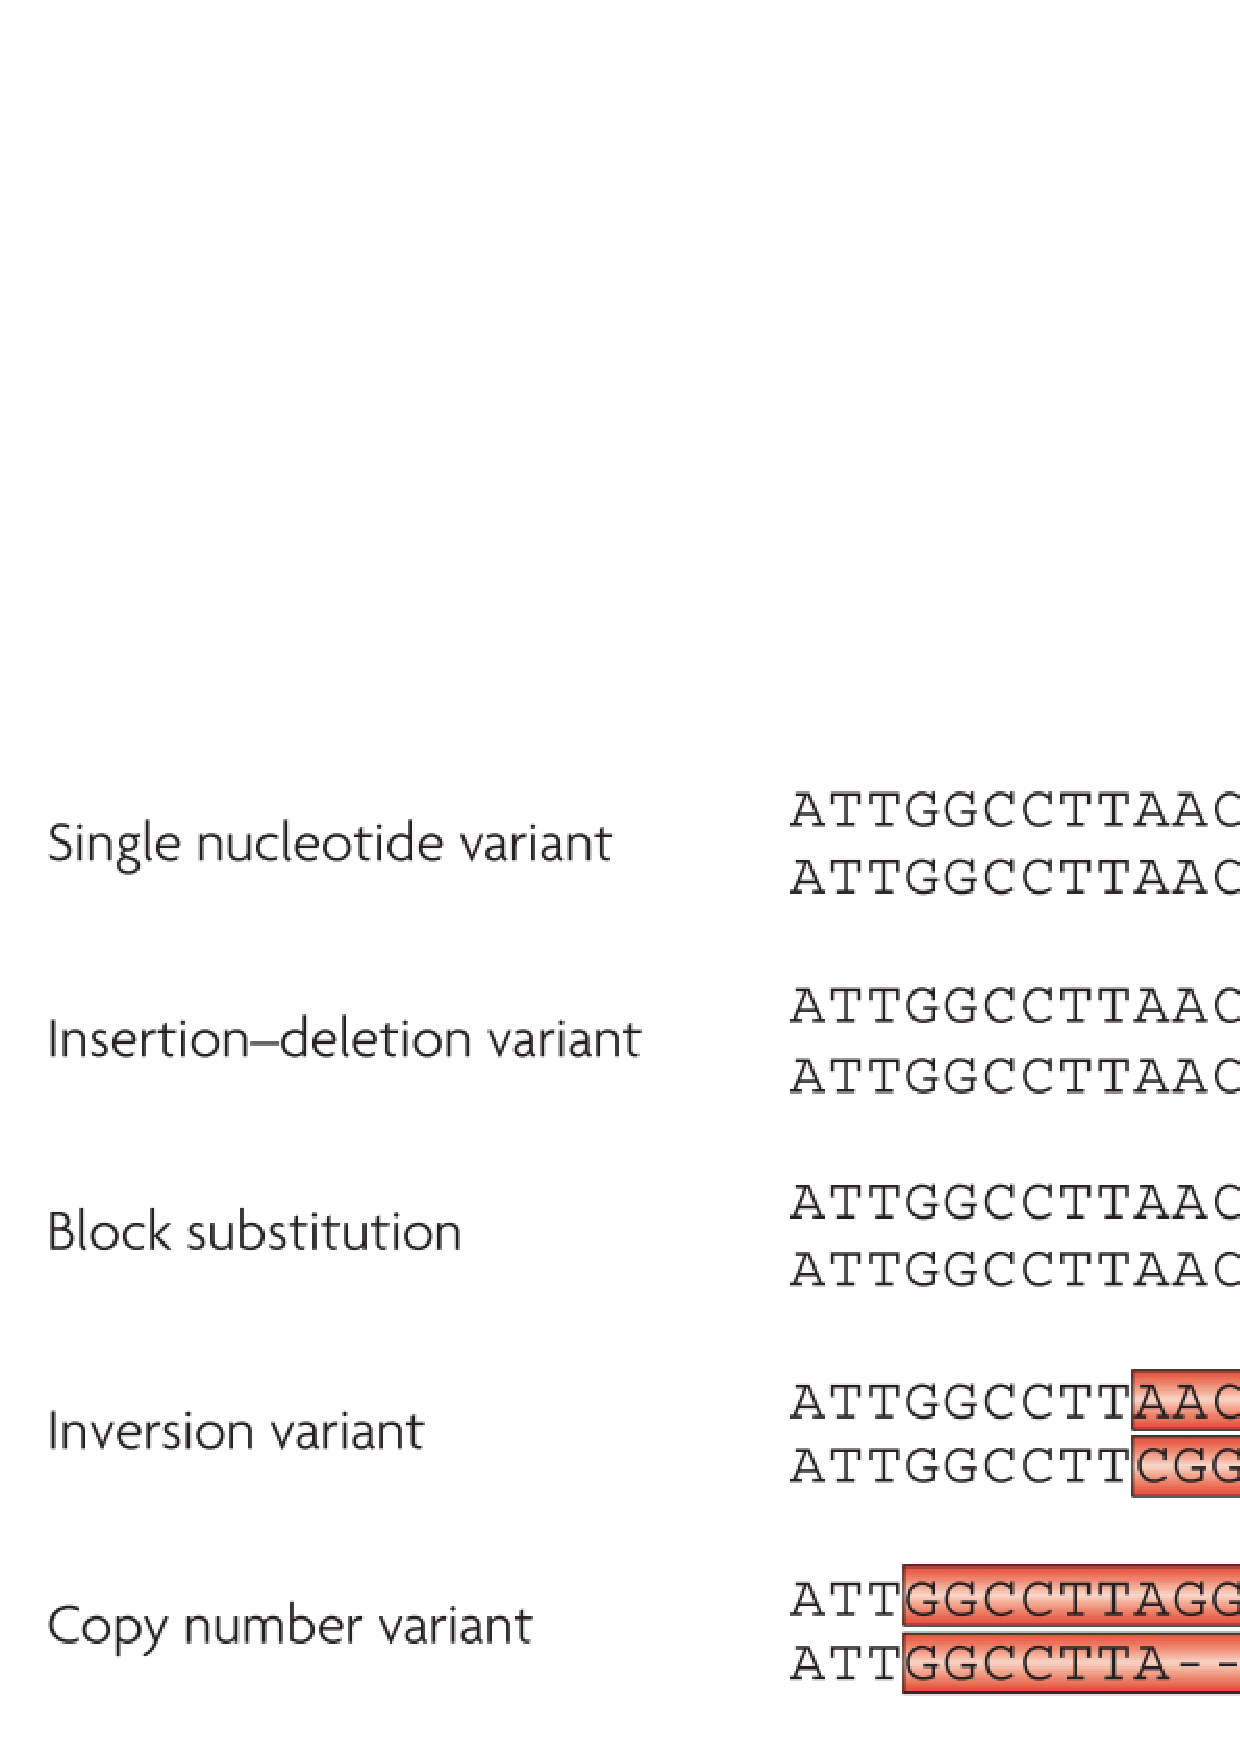
\includegraphics[width=0.3\textwidth]{/home/jennifer/Documentos/latex1/Plantilla_LaTex_UN/Kap4/variantes.png}
	\caption{Distribution of age range and gender of patients}
	\label{f:generosgeneral}
\end{figure}

\begin{figure}[h!]
	\centering
	\includegraphics[width=0.3\textwidth]{/home/jennifer/Documentos/latex1/Plantilla_LaTex_UN/Kap4/edad.png}
	\caption{Distribution of age range and gender of patients}
	\label{f:variantesgeneral}
\end{figure}





\subsubsection*{Sub-sub heading for section}
Text for this sub-sub-heading \ldots
\paragraph*{Sub-sub-sub heading for section}
Text for this sub-sub-sub-heading \ldots
In this section we examine the growth rate of the mean of $Z_0$, $Z_1$ and $Z_2$. In
addition, we examine a common modeling assumption and note the
importance of considering the tails of the extinction time $T_x$ in
studies of escape dynamics.
We will first consider the expected resistant population at $vT_x$ for
some $v>0$, (and temporarily assume $\alpha=0$)

$
 E \bigl[Z_1(vT_x) \bigr]= E
\biggl[\mu T_x\int_0^{v\wedge
1}Z_0(uT_x)
\exp \bigl(\lambda_1T_x(v-u) \bigr)\,du \biggr].$

If we assume that sensitive cells follow a deterministic decay
$Z_0(t)=xe^{\lambda_0 t}$ and approximate their extinction time as
$T_x\approx-\frac{1}{\lambda_0}\log x$, then we can heuristically
estimate the expected value as
%
\begin{eqnarray}\label{eqexpmuts}
E\bigl[Z_1(vT_x)\bigr] &=& \frac{\mu}{r}\log x
\int_0^{v\wedge1}x^{1-u}x^{({\lambda_1}/{r})(v-u)}\,du
\nonumber\\
&=& \frac{\mu}{r}x^{1-{\lambda_1}/{\lambda_0}v}\log x\int_0^{v\wedge
1}x^{-u(1+{\lambda_1}/{r})}\,du
\nonumber\\
&=& \frac{\mu}{\lambda_1-\lambda_0}x^{1+{\lambda_1}/{r}v} \biggl(1-\exp \biggl[-(v\wedge1) \biggl(1+
\frac{\lambda_1}{r}\biggr)\log x \biggr] \biggr).
\end{eqnarray}
%
Thus we observe that this expected value is finite for all $v>0$ (also see \cite{koon,khar,zvai,xjon,marg}).
%\nocite{oreg,schn,pond,smith,marg,hunn,advi,koha,mouse}

%%%%%%%%%%%%%%%%%%%%%%%%%%%%%%%%%%%%%%%%%%%%%%
%%                                          %%
%% Backmatter begins here                   %%
%%                                          %%
%%%%%%%%%%%%%%%%%%%%%%%%%%%%%%%%%%%%%%%%%%%%%%

\begin{backmatter}

\section*{Competing interests}
  The authors declare that they have no competing interests.

\section*{Author's contributions}
    Text for this section \ldots

\section*{Acknowledgements}
  Text for this section \ldots
%%%%%%%%%%%%%%%%%%%%%%%%%%%%%%%%%%%%%%%%%%%%%%%%%%%%%%%%%%%%%
%%                  The Bibliography                       %%
%%                                                         %%
%%  Bmc_mathpys.bst  will be used to                       %%
%%  create a .BBL file for submission.                     %%
%%  After submission of the .TEX file,                     %%
%%  you will be prompted to submit your .BBL file.         %%
%%                                                         %%
%%                                                         %%
%%  Note that the displayed Bibliography will not          %%
%%  necessarily be rendered by Latex exactly as specified  %%
%%  in the online Instructions for Authors.                %%
%%                                                         %%
%%%%%%%%%%%%%%%%%%%%%%%%%%%%%%%%%%%%%%%%%%%%%%%%%%%%%%%%%%%%%

% if your bibliography is in bibtex format, use those commands:
\bibliographystyle{bmc-mathphys} % Style BST file (bmc-mathphys, vancouver, spbasic).
\bibliography{library}      % Bibliography file (usually '*.bib' )
% for author-year bibliography (bmc-mathphys or spbasic)
% a) write to bib file (bmc-mathphys only)
% @settings{label, options="nameyear"}
% b) uncomment next line
%\nocite{label}

% or include bibliography directly:
% \begin{thebibliography}
% \bibitem{b1}
% \end{thebibliography}

%%%%%%%%%%%%%%%%%%%%%%%%%%%%%%%%%%%
%%                               %%
%% Figures                       %%
%%                               %%
%% NB: this is for captions and  %%
%% Titles. All graphics must be  %%
%% submitted separately and NOT  %%
%% included in the Tex document  %%
%%                               %%
%%%%%%%%%%%%%%%%%%%%%%%%%%%%%%%%%%%

%%
%% Do not use \listoffigures as most will included as separate files

\section*{Figures}
  \begin{figure}[h!]
  \caption{\csentence{Sample figure title.}
      A short description of the figure content
      should go here.}
      \end{figure}

\begin{figure}[h!]
  \caption{\csentence{Sample figure title.}
      Figure legend text.}
      \end{figure}

%%%%%%%%%%%%%%%%%%%%%%%%%%%%%%%%%%%
%%                               %%
%% Tables                        %%
%%                               %%
%%%%%%%%%%%%%%%%%%%%%%%%%%%%%%%%%%%

%% Use of \listoftables is discouraged.
%%
\section*{Tables}
\begin{table}[h!]
\caption{Sample table title. This is where the description of the table should go.}
      \begin{tabular}{cccc}
        \hline
           & B1  &B2   & B3\\ \hline
        A1 & 0.1 & 0.2 & 0.3\\
        A2 & ... & ..  & .\\
        A3 & ..  & .   & .\\ \hline
      \end{tabular}
\end{table}

%%%%%%%%%%%%%%%%%%%%%%%%%%%%%%%%%%%
%%                               %%
%% Additional Files              %%
%%                               %%
%%%%%%%%%%%%%%%%%%%%%%%%%%%%%%%%%%%

\section*{Additional Files}
  \subsection*{Additional file 1 --- Sample additional file title}
    Additional file descriptions text (including details of how to
    view the file, if it is in a non-standard format or the file extension).  This might
    refer to a multi-page table or a figure.

  \subsection*{Additional file 2 --- Sample additional file title}
    Additional file descriptions text.


\end{backmatter}
\end{document}
